\vspace{\baselineskip} 
\begin{itemize} 
\item To answer question 1, a literature review was conducted to identify the current trends in the space. Legacy rules-based analysis relied on the table data structure within relational databases and pre-defined thresholds for identifying potential fraudulent
transactions. Transactions over ten thousand dollars must be reported to the IRS. The key component that was missing from these systems was the ability to easily view the context of the transactions and the accounts that money is being transferred from or to.
As graph analytics\cite{GraphAnalytics} have evolved due to the rise of social networks, the financial industry has also embraced graphs to model financial transactions as a series of relationships to provide the missing context. Based on the literature review, we decided to utilize the graph data structure to model our data. Given the need to store, query, and visualize graph data, the data was converted
\cite{Neo4j}into nodes and edges via a Python script and imported into a graph database (Neo4j) that can natively handle the relationships and provide an efficient query mechanism.


\begin{figure}[H]
\begin{center}
    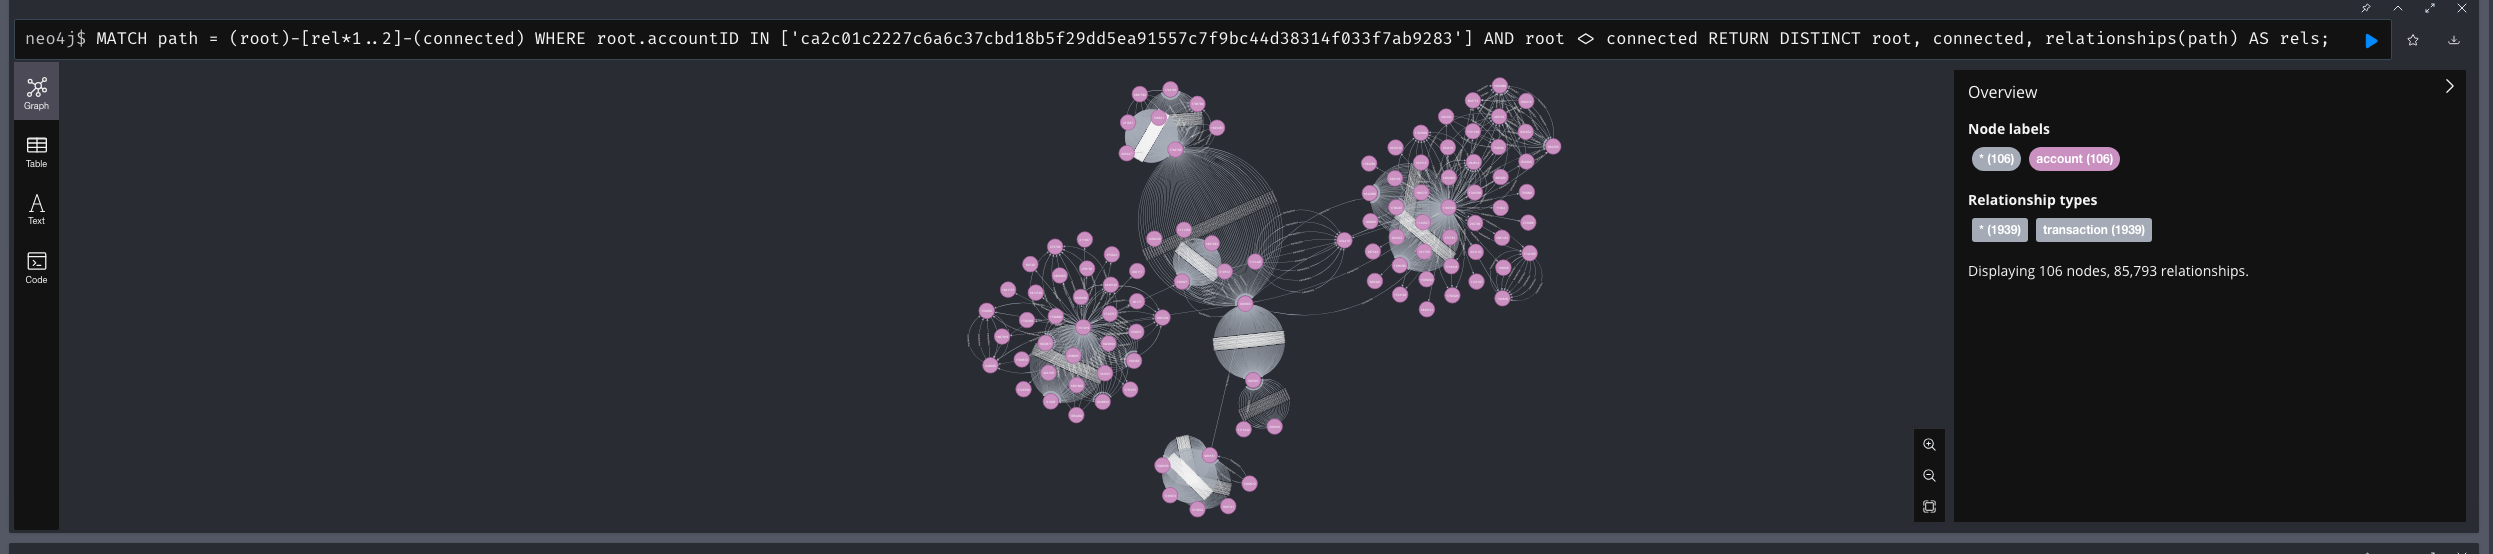
\includegraphics[width=8cm]{imgs/neo4j.png}
    \caption{Neo4j Database}
    \centering
\end{center}
\end{figure}

\item To answer question 2, the main issue to address was the screen bottleneck. With massive graph networks, the analyst can not visualize or analyze the graph using a traditional visualization. Despite this, analysts will need to perform an ad-hoc review of accounts to identify potential accounts of interest. Visualizing the data with a graph city solves this problem by allowing analysts to
see the entire graph and perform analysis one building at a time. We used the graph city architecture introduced by James Abello, H. Zhang, Daniel Nakhimovich, Chengguizi Han, and Mridul Aanjaneya.\cite{Abello2022GigaGC}\cite{Abello2021GraphCT}\cite{Abello2020GraphW}\cite{Abello2013FixedPO}

\begin{figure}[htp]
    \centering
    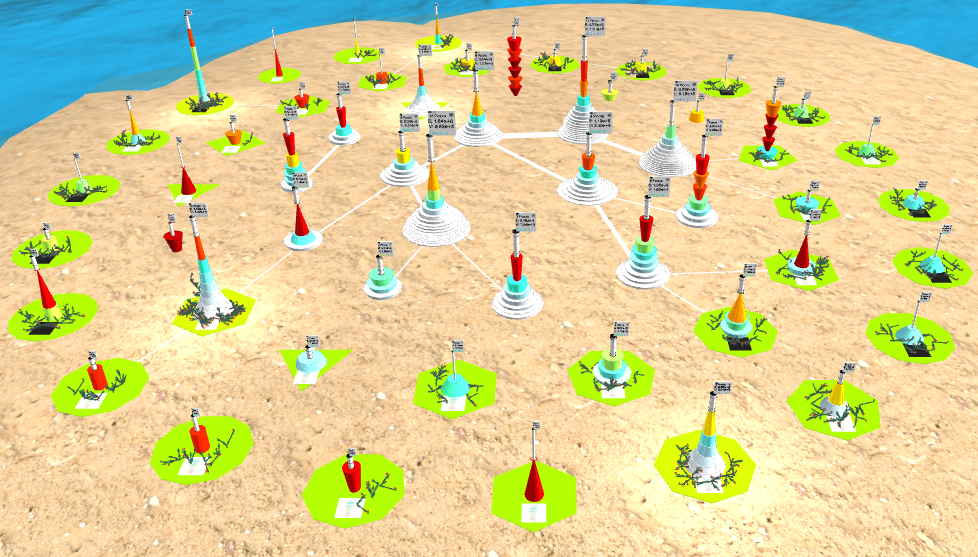
\includegraphics[width=7cm]{imgs/graph_city.png}
    \caption{Graph City Buildings}
    \label{fig:DataFlowDiagram}
\end{figure}


\begin{figure}[H]
\begin{center}
    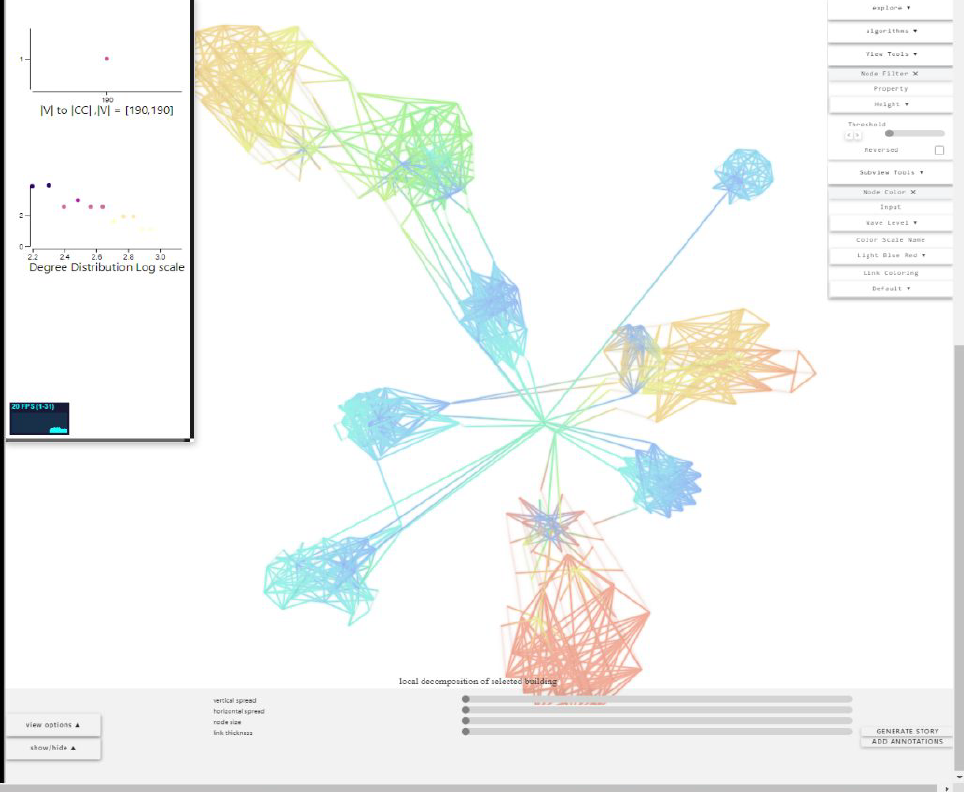
\includegraphics[width=7cm]{imgs/graph_node.png}
    \caption{Graph Nodes}
    \centering
\end{center}
\end{figure}

\item To answer question 3, we needed to figure out how to leverage Neo4j's advanced capabilities to allow analysts to view transactions for particular accounts and their related accounts. This was done by creating a search application that allows the user to filter on
certain key attributes and visualize a graph of an account (or series of accounts).

\begin{figure}[H]
\begin{center}
    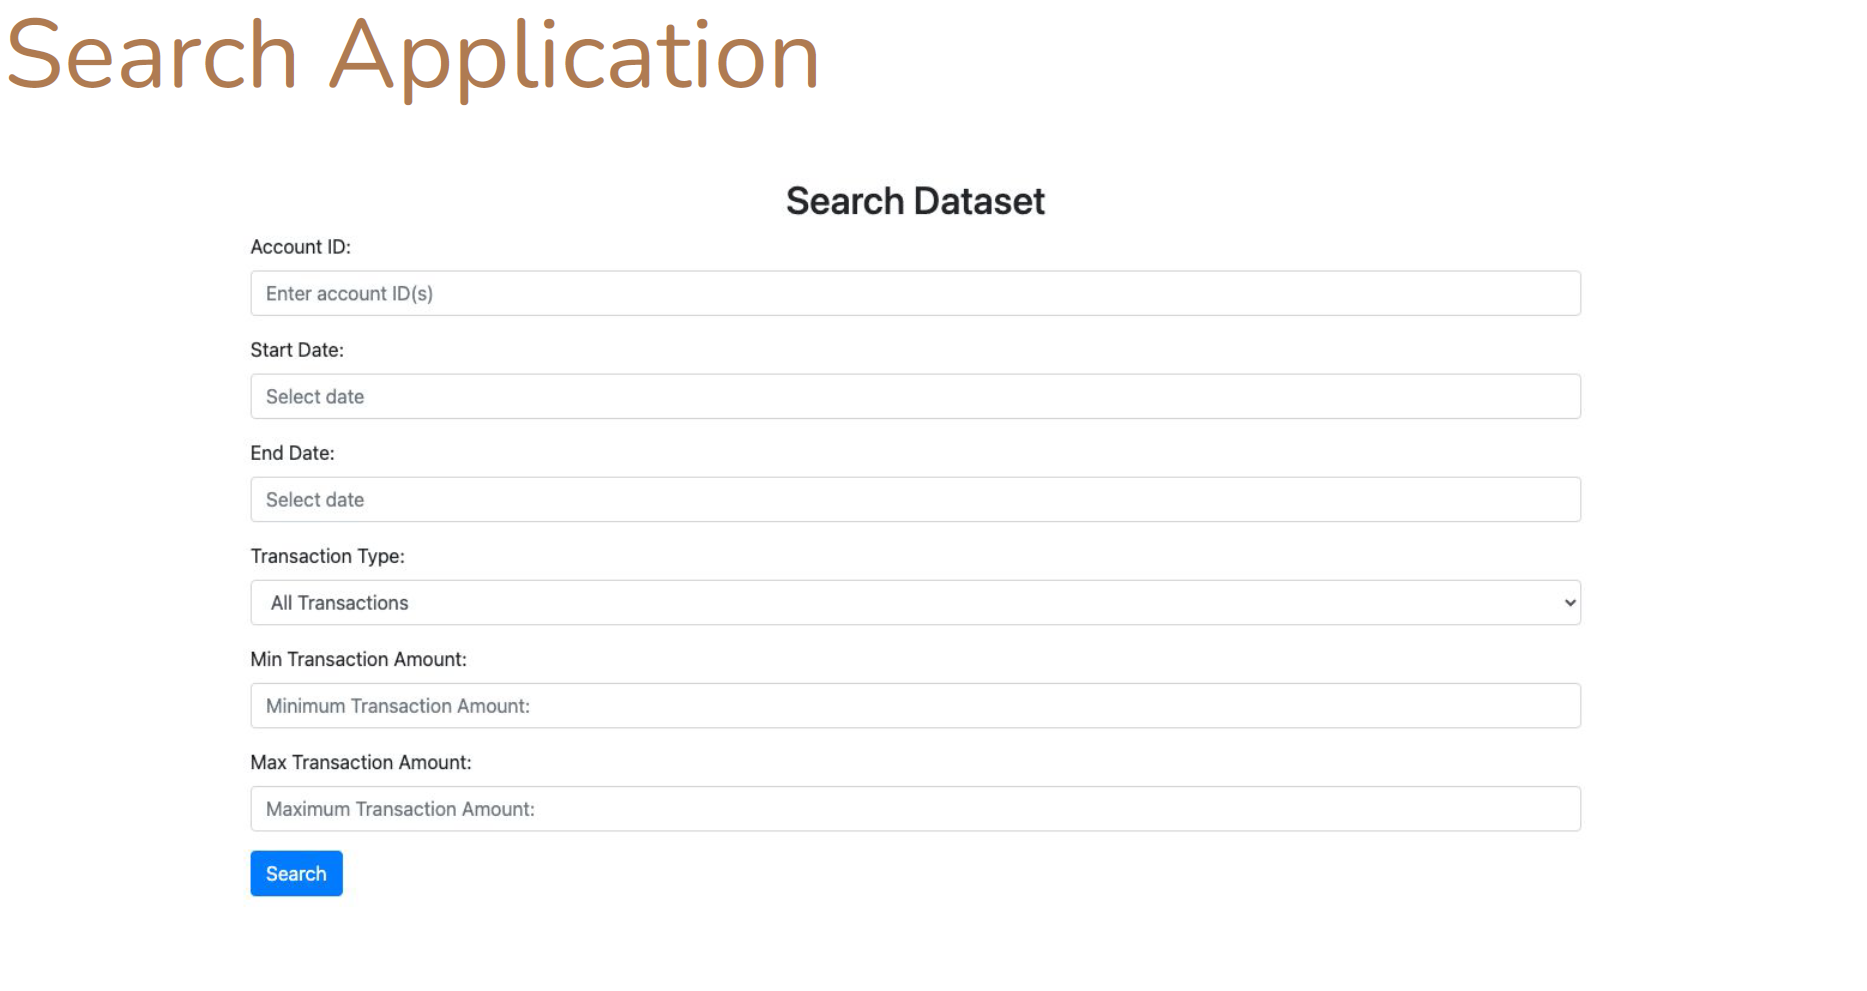
\includegraphics[width=8cm]{imgs/searchapp.png}
    \caption{Search Application}
    \centering
\end{center}
\end{figure}

Once the query is submitted, a graph visualization is rendered that shows all transactions by that account and also any transaction by accounts that the account sent money to (depth 2).\cite{Neovis}

\begin{figure}[H]
\begin{center}
    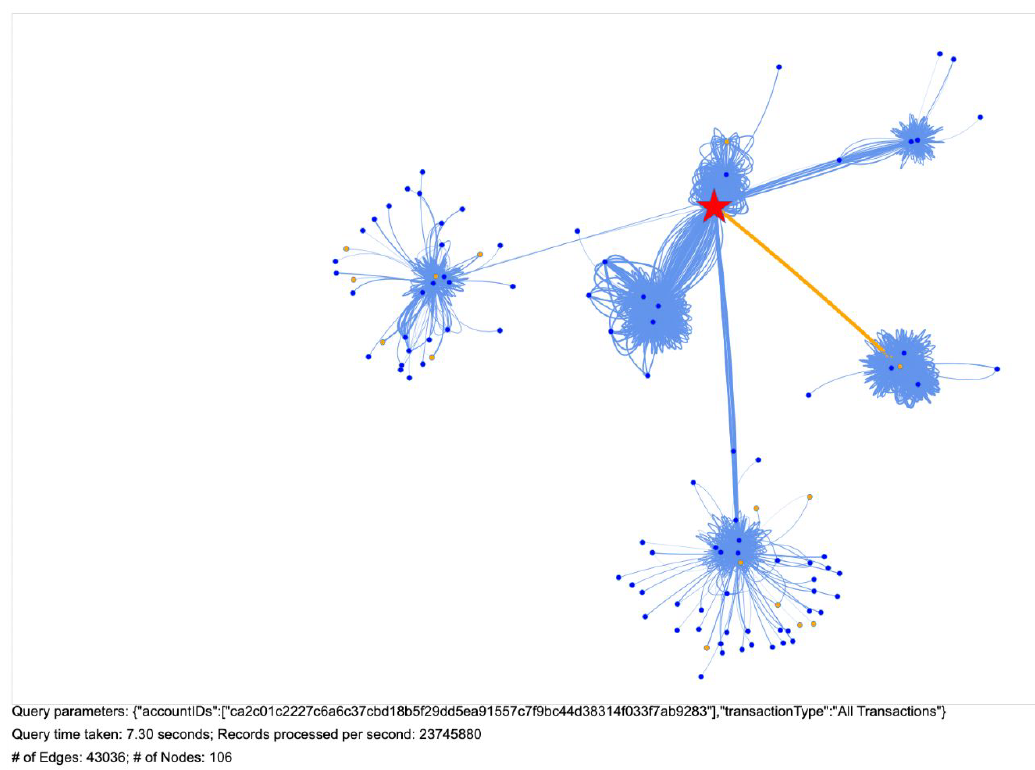
\includegraphics[width=8cm]{imgs/queryresult.png}
    \caption{Query Result}
    \centering
\end{center}
\end{figure}

An interesting finding is that communities of interest are readily apparent when visualizing the accounts through the search application.


\end{itemize}

